\documentclass{article}
%\usepackage{psfig}
\usepackage[margin=1.25in]{geometry}
\usepackage{amsmath}
\usepackage{amssymb}
\usepackage{enumerate}
\usepackage{hyperref}
\usepackage{graphicx}

\pagestyle{empty}

\newcommand{\points}[1]{\mbox{\textbf{[#1 Points]}}}
\newcommand{\extracredit}{\mbox{\textbf{[Extra Credit]}}}

\begin{document}

\title{CS181 Assignment 1: Decision Trees}
\author{Professor David Parkes\\\\Out Monday, January 31st\\Due at
  Noon of Friday, February 11th}

\maketitle

\noindent General Instructions:

You may work with one other person on this assignment.
Each group should turn in one writeup. To submit, copy your assignment
files to \verb=nice.fas.harvard.edu= and run \verb=make submit=.
This assignment consists of a theoretical component and an experimental
component.  The experimental component requires you to write code and
analyze the effectiveness
of different algorithms you implement.  For the experimental results,
we have provided a graphical interface that will generate the
requisite charts and figures from your code.\\

In this assignment, you will develop a classifier for medical data.  You will be working with a
database of instances describing patients who have been tested for breast cancer.
You will develop a classifier that can classify growths as
malignant or benign, based on the results of tests taken by a patient.
The dataset was derived from the Wisconsin breast cancer corpus,
obtained from the UC Irvine machine learning repository at \url{http://archive.ics.uci.edu/ml/}.
The UC Irvine repository is an important collection of many of the
most frequently used machine learning benchmarks.

You can find the dataset for this assignment, as well as code, at
\url{http://www.seas.harvard.edu/courses/cs181/docs/asst1.tar.gz}.  The data can
be found in \verb@data.csv@, while \verb@noisy.dat@ contains the same data with a certain amount of
random ``noise'' added.  Each dataset contains a total of 100 samples.  Each sample in the data
consists of 9 features, each of which ranges from 1 to 10, and a boolean classification that is 0 or
1.  The file \verb@breast-cancer-wisconsin.names@ describes the features and also contains
information about the history of the dataset.

\begin{enumerate}
\item \points{15} \textbf{Decision Trees and ID3}

\begin{enumerate}
\item \points{5}
Suppose that the ID3 algorithm is in the middle of classifying a data
set, and there are seven instances remaining, with four positive and
three negative instances.  It has the choice of splitting on two
binary features $A$ and $B$.  When $A$ is true, there are two
positive and two negative instances, while when $A$ is false, there
are two positive and one negative instances.  Meanwhile, when $B$ is
true there is one positive and one negative instance, while when $B$
is false there are three positive and two negative instances.

Which feature will ID3 choose to split on?  Show the information
gain calculations.
For each of the two possible splits, present an informal and brief
argument that the split is more useful than the other.  What does this
example show about the inductive bias of ID3?

\item \points{5}

Use your work in part~(a) to show a tree that ID3 might construct for
the following dataset, in which there are four Boolean features and
a Boolean classification.  You do not need to show the information gain
computations, but you should briefly justify why a particular
feature was chosen at each point in the tree.  In case a tie needs
to be broken, indicate which other feature(s) could have been chosen.

\centerline{
\begin{tabular}{|c|c|c|c|c|}
\hline
A & B & C & D & Class \\
\hline\hline
T & F & T & F & F \\
T & F & F & F & T \\
F & F & F & T & F \\
T & F & F & T & T \\
F & T & T & T & T \\
T & T & F & T & F \\
F & F & F & T & T \\
\hline
\end{tabular}
}

\item \points{5}
By eyeballing the data, find a simpler tree that has the same training
error as the one produced by ID3.  What can we learn from this
example about the ID3 algorithm?
\end{enumerate}

\item \points{77} \textbf{ID3 with Pruning}

In this section, we will implement the following machine learning techniques:
\begin{itemize}
\item ID3
\item bottom-up decision tree pruning
\item cross-validation
\item AdaBoost (to be covered in class on Wednesday, February 2nd)
\end{itemize}

This will require a substantial amount of code. We've provided you
with a few resources. You should begin by downloading the assignment
code here:
\url{http://www.seas.harvard.edu/courses/cs181/docs/asst1.tar.gz}\\
You can extract this archive with \verb=tar -xvzf asst1.tar.gz= on
Linux or OS X. On Windows, we recommend you use
\href{http://www.7-zip.org/}{7-Zip} to extract the archive.

This portion of the assignment will consist of a series of programming
exercises. As you complete the exercises, you will be able to answer a
series of accompanying questions. You should include your answers in
the written portion of the assignment. These questions have been
marked a double arrow like this:

$\Rightarrow$ \href{http://books.google.com/books?id=\_0YB05NPhJUC\&pg=PA34\&lpg=PA34\&dq=catch+22+who+is+spain+why+is+hitler\&source=bl\&ots=647YrqxwpY\&sig=PT4udMwGjMMJS2AtqpNDP-sopw0\&hl=en\&ei=q\_FFTeOqKMOqlAef4fgf\&sa=X\&oi=book\_result\&ct=result\&resnum=2\&ved=0CCMQ6AEwAQ\#v=onepage\&q\&f=false}{Who is Spain?}\\

To help you with this assignment, we
have provided a number of empty python functions for you to fill
in. You should be able to get an idea of what each function does by
looking at it's {\em docstring}, which is a special comment beginning
on the line below the function name.\\

Furthermore, we have provided you with an extensive test suite to
exercise your code. This test suite contains a set of {\em unit
  tests}. A unit test is piece of code designed to exercise an atomic
piece or ``unit'' of code and ensure its proper functionality. Unit
testing a piece of code allows you to find bugs earlier and build on
top of existing code with confidence. To (optionally) read more about
unit testing, check out Wikipedia's excellent article on the subject:
\href{http://en.wikipedia.org/wiki/Unit_testing}.

You can run the test suite on the command line
(\verb=python testdtree.py=), or through a handy web interface that
runs in your browser. To use this interface, run \verb=./hw1= on Linux
of OS X, or \verb=hw1.bat= on Windows. (Note: the \verb=.bat= file has
not been tested. You should contact
\href{mailto:cs181@fas.harvard.edu} if you have trouble starting the
graphical interface on Windows.) 

\begin{center}
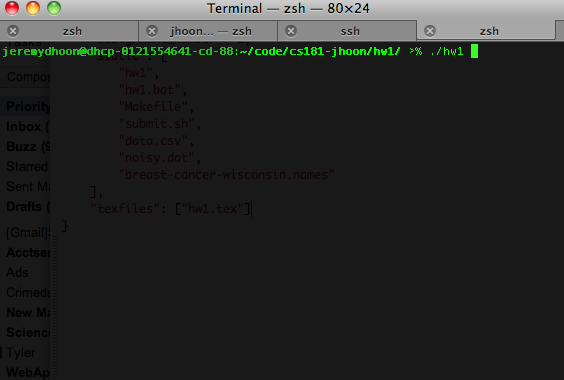
\includegraphics[width=125mm]{running_webface.png}
\end{center}

This should bring up the interface:

\begin{center}
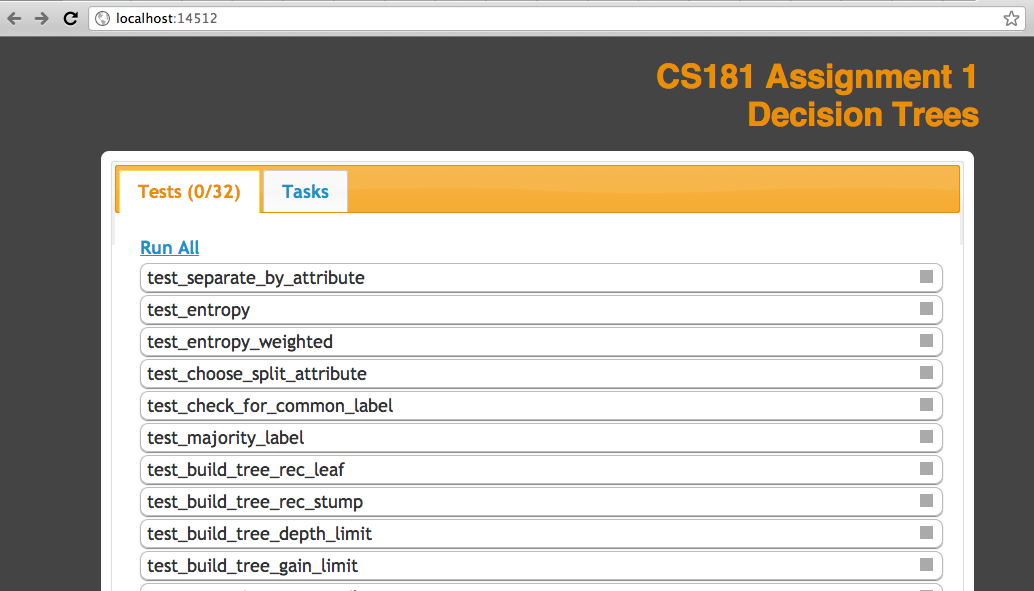
\includegraphics[width=125mm]{test_screen.png}
\end{center}

Clicking on the name of any test will run it. If the test passes, the
square on the right side of the test name will turn green. If the test
fails, the square will turn red, and a button titled ``Show Failure''
will appear. Clicking this button will reveal a traceback that may
contain information about the test failure.\\

The idea behind testing is that it will allow you to quickly build on
your work and reduce the amount of time you will spend debugging. In
order to help you see how the functions you're implmenting fit
together, we've included a call graph from the solution code. It is
contained in the file \verb=call_graph.png=.

As a warmup, implement the function in \verb=dtree.py= called
\verb=compute_entropy=. An explanation of this function is provided in
its docstring. In the web interface, run the
\verb=test_compute_entropy= test. Once your function is working and
the test passes, open up your web interface,
click the ``Tasks'' tab, and then find the task called ``Plot Entropy
Curve.'' It should be the first task on the list. Click ``Run.'' This
should generate an entropy curve like that shown in the lecture
notes. As you progress through this assignment, you will be able to
run the rest of the tasks in the ``Tasks'' pane. If run you a task that
relies on functionality you have not yet implemented, or if your code
raises an exception, you will see a stack trace which provides the
details of the exception.

\begin{enumerate}
\item \points{20} First up, we'll be implementing ID3. Open up
  \verb#dtree.py#. Complete the following functions:
  \begin{itemize}
    \item \verb=separate_by_attribute=
    \item \verb=compute_entropy_of_split=
    \item \verb=choose_split_attribute=
    \item \verb=check_for_common_label=
    \item \verb=majority_label=
    \item \verb=build_tree_rec=
    \item \verb=count_instance_attributes=
    \item \verb=classify=
  \end{itemize}
Most of these functions will be quite short, often less than ten
lines. Whenever possible, try to use functionality you have already
implememented by calling a function you have already filled-in and
tested. For a hint as to which functions you might find useful in
implementing function \verb=foo=, look at the solution code call
graph, locate the box for \verb=foo=, and see which functions it
calls. Once you've implemented a function, run any corresponding tests
for that function and make sure they pass.\\

When you've implemented these functions, you will be ready to run
another task. Find the
task called ``Build BCW Tree,'' and click ``Run.'' This should produce
a visualization of a decision tree built from the BCW dataset.

\begin{center}
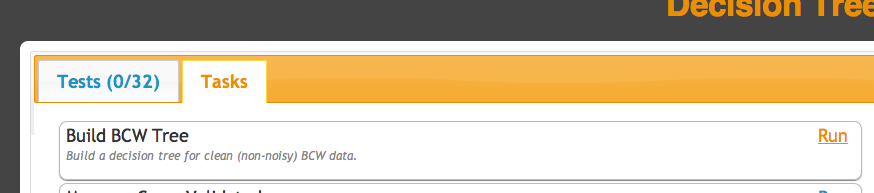
\includegraphics[width=125mm]{first_task.png}
\end{center}

Note: In order to build decision trees (using the \verb=DTree= class)
you may find it easiest to use Python's {\em keyword argument}
feature, explained here:
\url{http://docs.python.org/tutorial/controlflow.html#keyword-arguments}

\item \points{10}

As a prelude to pruning, we need to implement
cross-validation. This functionality is encompassed by the following
functions:

\begin{itemize}
\item \verb=weight_correct_incorrect=
\item \verb=evaluate_classification=
\item \verb=check_folds=
\item \verb=yield_cv_folds=
\item \verb=cv_score=
\end{itemize}

When you've completed these functions, you should be able to run the
next two tasks: ``Measure Cross-Validated ID3 Training Set Accuracy'' and
``Measure Cross-Validated Performance.'' The first task will
demonstrate the training set accuracy of ID3 without prunung. The
second task will give you
cross-validated test performance on both the clean and noisy data
sets. 

\item \points{15} Now on to validation-set pruning. In order to get
  this working, you'll need to figure out how to implement
  cross-validation with a validation set. You'll need to implement the
  following:

  \begin{itemize}
    \item \verb=prune_tree=
    \item \verb=build_pruned_tree=
    \item \verb=yield_cv_folds_with_validation=
  \end{itemize}

  You should be able to re-run the task named ``Measure
  Cross-Validated Performance.'' and see results for pruned decision
  trees. You can also see the result of validation set pruning on a
  decision tree for the BCW data set when you run ``Prune BCW Decision
  Tree.''

  $\Rightarrow$ Does ID3 suffer from overfitting on this data set?
  Justify your answer.

\item \points{32} \textbf{Boosting}

The boosting paradigm presents another way of overcoming the
over-fitting problem.  In this problem,
you will implement AdaBoost and experiment with various different
boosting possibilities.

Remember that AdaBoost builds a series of classifiers from the same
learner. In each round of boosting, AdaBoost changes the weight it
places on the various instances in its training set. As preparation
for this aspect of the algorithm, the ID3 functionality you have
implemented up to this point has taken instance weight into
account. For example, splitting decisions (in
\verb=choose_split_attribute=) and cross-validated accuracy
calcuations (\verb=cv_score=) required you to consider the weights of
the instances involved in these operations.

\begin{enumerate}
\item $\Rightarrow$ \points{4} How does your ID3
implementation make use of instance weight in the splitting decisions
it makes? Explain why AdaBoost on ID3 would not work if splitting decisions
in ID3 were made by counting instances rather than summing weights.

 \item $\Rightarrow$ \points{4} What is the weighted entropy of a set of examples
   $\{\mathbf{x_1}, \ldots, \mathbf{x_n}\}$ where target $y_1 =
T$ but all other targets $y_i = F$ and $w_1 = 0.5$ while all other
weights are $0.5 / (n - 1)$?
\end{enumerate}

Now, complete the following functions in order to implement boosting:
\begin{itemize}
\item \verb=normalize_weights=
\item \verb=init_weights=
\item \verb=classifier_error=
\item \verb=classifier_weight=
\item \verb=update_weight_unnormalized=
\item \verb=one_round_boost=
\item \verb=boost=
\item \verb=classify_boosted=
\item \verb=yield_boosted_folds=
\end{itemize}

Once you've completed these functions, you should be able to run all
remaining tasks. Using the charts produced by these tasks, answer the
following questions in your written response:

\begin{enumerate}
\item $\Rightarrow$ \points{6} Compare the effectiveness
of boosting to the other methods you implemented previously. What do
the relative performances of pruned decision trees and boosting on the
noisy data set imply about types of classification problems in which
boosting is effective?
\item $\Rightarrow$ \points{6} How does the maximum depth of the weak
  learner affect 
  cross-validated test performance for boosting on both datasets?  How
  can we explain these results?
\item $\Rightarrow$ \points{6} If we did not know that boosting
  produces a maximum-margin 
  classifier, what would we find surprising in comparing the results
  from 10 and 30 rounds of boosting?
\item $\Rightarrow$ \points{6} What is the relationship between training- and test-set
  cross-validation performance over the first fifteen rounds of
  boosting?
\end{enumerate}

\end{enumerate}

\item \points{8} \textbf{Tree Analysis}\\
Choose a particularly effective decision tree on the BCW data set and
examine the structure of the tree, mapping
feature indices to qualitative descriptions using the file
\verb=breast-cancer-wisconsin.names=.
Present the tree you choose along with the methodology used to generate the tree.
Which features are most important for benign / malignant
determination?

\end{enumerate}
\end{document}

